\tikzstyle{pvalue}=[circle, draw, fill=blue!50, minimum height=3em]
\tikzstyle{ovalue}=[circle, draw,fill=red!50, minimum height=3em]
\tikzstyle{dcell}=[circle,draw, minimum height=1em]
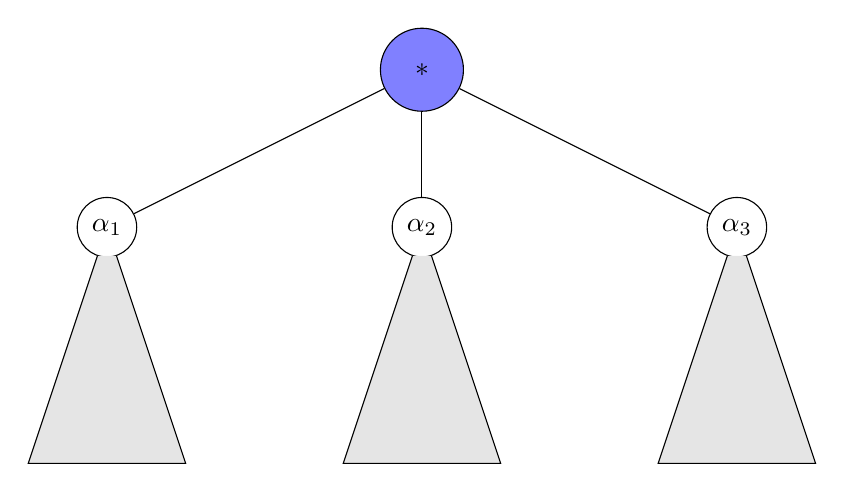
\begin{tikzpicture}

\node[dcell] (v3) at (8,1) {$\alpha_3$};
\draw[draw,fill=gray!20] (v3) -- (7,-2) -- (9,-2) -- (v3) -- cycle;


\node[dcell] (v2) at (4,1) {$\alpha_2$};
\draw[draw,fill=gray!20] (v2) -- (3,-2) -- (5,-2) -- (v2) -- cycle;

\node[dcell] (v1) at (0,1) {$\alpha_1$};
\draw[draw,fill=gray!20] (v1) -- (-1,-2) -- (1,-2) -- (v1) -- cycle;
\node[pvalue] (v5) at (4,3) {$\Large{*}$};
\draw  (v5) edge (v1);
\draw  (v5) edge (v2);
\draw  (v5) edge (v3);
\end{tikzpicture}